%% LyX 2.3.1 created this file.  For more info, see http://www.lyx.org/.
%% Do not edit unless you really know what you are doing.
\documentclass[11pt,english,openright]{book}
\usepackage[T1]{fontenc}
\usepackage[latin9]{inputenc}
\usepackage[a4paper]{geometry}
\geometry{verbose,tmargin=3cm,bmargin=3.5cm,lmargin=4cm,rmargin=3cm}
\setcounter{secnumdepth}{3}
\setcounter{tocdepth}{3}
\usepackage{color}
\usepackage{babel}
\usepackage{float}
\usepackage{booktabs}
\usepackage{url}
\usepackage{amsmath}
\usepackage{amssymb}
\usepackage{graphicx}
\usepackage{setspace}
\onehalfspacing
\usepackage[unicode=true,pdfusetitle,
 bookmarks=true,bookmarksnumbered=false,bookmarksopen=false,
 breaklinks=false,pdfborder={0 0 1},backref=false,colorlinks=false]
 {hyperref}

\makeatletter

%%%%%%%%%%%%%%%%%%%%%%%%%%%%%% LyX specific LaTeX commands.
\providecommand{\LyX}{\texorpdfstring%
  {L\kern-.1667em\lower.25em\hbox{Y}\kern-.125emX\@}
  {LyX}}
\DeclareRobustCommand*{\lyxarrow}{%
\@ifstar
{\leavevmode\,$\triangleleft$\,\allowbreak}
{\leavevmode\,$\triangleright$\,\allowbreak}}
%% Because html converters don't know tabularnewline
\providecommand{\tabularnewline}{\\}
\floatstyle{ruled}
\newfloat{algorithm}{tbp}{loa}[chapter]
\providecommand{\algorithmname}{Algorithm}
\floatname{algorithm}{\protect\algorithmname}

%%%%%%%%%%%%%%%%%%%%%%%%%%%%%% User specified LaTeX commands.
% additional packages
\usepackage{tabularx}
\usepackage{setspace}
\usepackage{amsthm}
\usepackage{rotating}
\usepackage{caption}
\usepackage{epsfig}
\usepackage{indentfirst}
\usepackage{fancyhdr}
\usepackage{url}
\usepackage{cite}
\usepackage[normalem]{ulem}
\usepackage[table]{xcolor}
\usepackage{booktabs}
\usepackage{algpseudocode}

% this is a dirty fix for LTS version of Ubuntu/Kubuntu that has a
% very outdated "geometry" package
\include{geometry.sty}

% fixes the page number of the first page of each chapter
\fancypagestyle{plain}{
\fancyhead{}
\renewcommand{\headrulewidth}{0pt}
\renewcommand{\footrulewidth}{0pt}
\fancyfoot[OC]{\begin{flushright}\thepage\end{flushright}}
}

% fancy headers for the thesis
\fancyhead{}
\fancyhead[LE]{\slshape \nouppercase \leftmark}
\fancyhead[RO]{\slshape \nouppercase \rightmark}
\fancyfoot[EC]{\begin{flushleft}\thepage\end{flushleft}}
\fancyfoot[OC]{\begin{flushright}\thepage\end{flushright}}
\renewcommand{\headrulewidth}{0.4pt}
\setlength{\headheight}{14pt}

\@ifundefined{showcaptionsetup}{}{%
 \PassOptionsToPackage{caption=false}{subfig}}
\usepackage{subfig}
\makeatother

\usepackage{listings}
\renewcommand{\lstlistingname}{Listing}

\begin{document}
\frontmatter
\pagestyle{empty}
\newgeometry{margin=3cm}\begin{titlepage}

\begin{center}
\Large{\textsc{Politecnico di Milano}}\\
\Large{Scuola di Ingegneria Industriale e dell'Informazione}\\
\large{Corso di Laurea Magistrale in Computer Science and Engineering}\\
\large{Ingegneria Informatica}
\par\end{center}

\vspace{0.5cm}

\begin{center}
\begin{figure}[h]
\centering{}
\includegraphics[width=0.3\textwidth]{title-page/logo-polimi}
\end{figure}
\vspace{1cm}
\par\end{center}

\begin{center}
\LARGE{GEA\\
Gioco Educazione Alimentare}\vspace{2cm}
\par\end{center}

\begin{flushleft}
\begin{tabular}{ll}
Relatore:  & Prof.ssa Franca GARZOTTO\tabularnewline
Correlatore:  & Dott. Mirko GELSOMINI\tabularnewline
\end{tabular}\vspace{1cm}
\par\end{flushleft}

\begin{flushright}
\begin{tabular}{ll}
Tesi di laurea di: & \tabularnewline
Federica BLANCO & Matr. 875487\tabularnewline
Giulia PENNATI & Matr. 882962\tabularnewline
\end{tabular}\vspace{4cm}
\par\end{flushright}

\begin{center}
{\large{}Anno Accademico 2017--2018}{\large\par}
\par\end{center}

\end{titlepage}
\restoregeometry

\cleardoublepage{}

\begin{flushright}
\emph{\input{dedication.tex}}\cleardoublepage{}
\par\end{flushright}

\chapter*{Acknowledgments}

\thispagestyle{empty}\input{acknowledgments.tex}\cleardoublepage{}

\chapter*{Abstract}

\thispagestyle{empty}\input{abstract.tex}\cleardoublepage{}

\chapter*{Sommario}

\thispagestyle{empty}In italiano, descrizione NDD, scopo tesi, descrizione tecnologia usata(in breve), nome sistema sviluppato e collaborazione. (circa 1 pagina)\cleardoublepage\pagenumbering{roman}
\setcounter{page}{1}
\pagestyle{fancy}\tableofcontents{}\listoffigures
\listoftables
\listof{algorithm}{List of Algorithms}
\cleardoublepage\mainmatter
\renewcommand{\sectionmark}[1]{\markright{\thesection.\ #1}}
\renewcommand{\chaptermark}[1]{\markboth{\thechapter.\ #1}{}}

\chapter*{Introduction\label{chap:introduction}}

\addcontentsline{toc}{chapter}{Introduction}
\markboth{Introduction}{Introduction}\emph{}

\section{Virtual Reality}
\section{NDD}
\section{GEA}
\subsection{Thesi Structure}
\subsection{Origin of the name}
logo



\chapter{First chapter\label{chap:first-chapter}}

\input{chapter-1/chapter-1.tex}

\chapter{Second chapter\label{chap:second-chapter}}

These are general tips about few \LaTeX{} and \LyX{} functionalities.

\section{Copy and paste raw \protect\LaTeX{} code}

Sometimes it is necessary to insert raw \LaTeX{} code in your document,
\LyX{} has a dedicated environment for that (\textsf{Insert} \textsf{\lyxarrow}
\textsf{Tex code}). By using the paste command (\textsf{CTRL + V})
to copy text into that type of environment, you get as result that
everything is copied in a single line, all the carriage returns are
ignored. To paste exactly what you have copied, use the special paste
command which preserves the text formatting (\textsf{CTRL + SHIFT
+ V} or \textsf{Edit} \textsf{\lyxarrow{} Paste Special \lyxarrow Plain
Text}).

\section{Labels and cross-references\label{sec:label-and-cross}}

Labels are necessary to add cross-references in your thesis, use a
label for each element that you have to reference to (\textsf{Insert}
\textsf{\lyxarrow} \textsf{Label/Cross-reference}). These elements
are manly chapters, sections, subsections, figures, tables and algorithms.

This is Chapter \ref{chap:second-chapter}, Section \ref{sec:label-and-cross}.

\section{Figures}

Figures, but also tables and algorithms, must be placed inside a floating
environment. This type of \LaTeX{} environment is very useful and automagically
mix up text and images. Usually the \textsf{Here if possible} placement
option is good for all images (right click on \textsf{float: Figure}
then \textsf{Settings}). However, if the figure is not placed correctly
you may enable the \textsf{Ignore \LaTeX{} rules} option, usually that
option solves every problem.

Figure \ref{fig:image} shows an example of a very nice animal.

\begin{figure}[h]
\begin{centering}
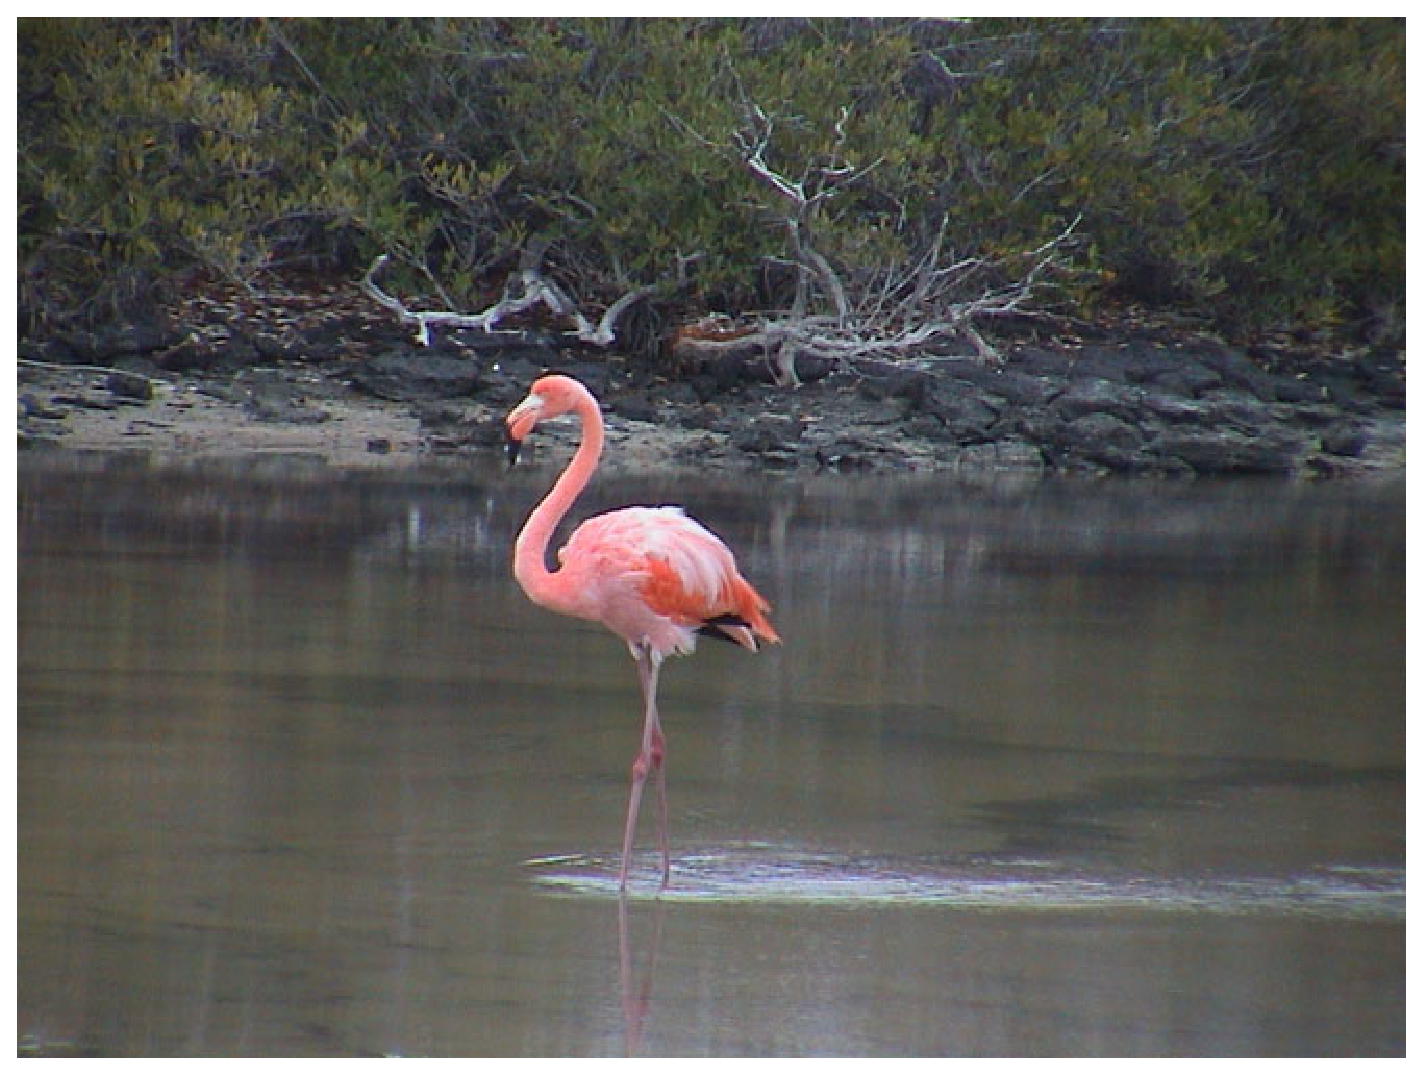
\includegraphics[width=0.5\columnwidth]{chapter-2/images/flamingo}
\par\end{centering}
\caption[Short caption of the figure]{\label{fig:image}Detailed caption of this marvelous animal}
\end{figure}
A rarely known feature of \LyX{} is the possibility to add the short
caption. The short caption is the description of the figure used in
the \textsf{List of Figures} section. Sometimes captions can be very
long, in this case it is better to use a shorter one that is more
readable in the page that lists all the figures. To add this caption,
right click on the description of figure, then \textsf{Insert short
title}.

It is not mandatory to add the short caption, it is only useful with
very long captions to ensure a better legibility of the \textsf{List
of Figures} section.

\subsection{Subfigures}

A very cool feature of \LaTeX 's figures is the possibility to have
subfigures. For example, if there are two figures that represent the
result of a test executed with two different values of a parameter,
then a subfigure is a good way to organize the images.

Figure \ref{fig:subfig-fauna} is an example of these subfigures.
References can be added to either the whole figure (Figure \ref{fig:subfig-fauna})
or each subfigure (Figure \ref{fig:fauna-squirrel} and Figure \ref{fig:fauna-peacock}).

\begin{figure}[h]
\hfill{}\subfloat[\label{fig:fauna-squirrel}A nice squirrel]{\centering{}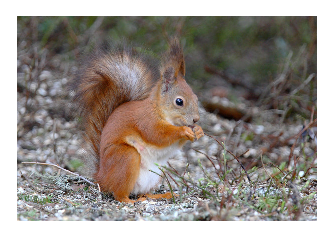
\includegraphics[width=0.45\columnwidth]{chapter-2/images/squirrel}}\hfill{}\subfloat[\label{fig:fauna-peacock}A beautiful peacock]{\centering{}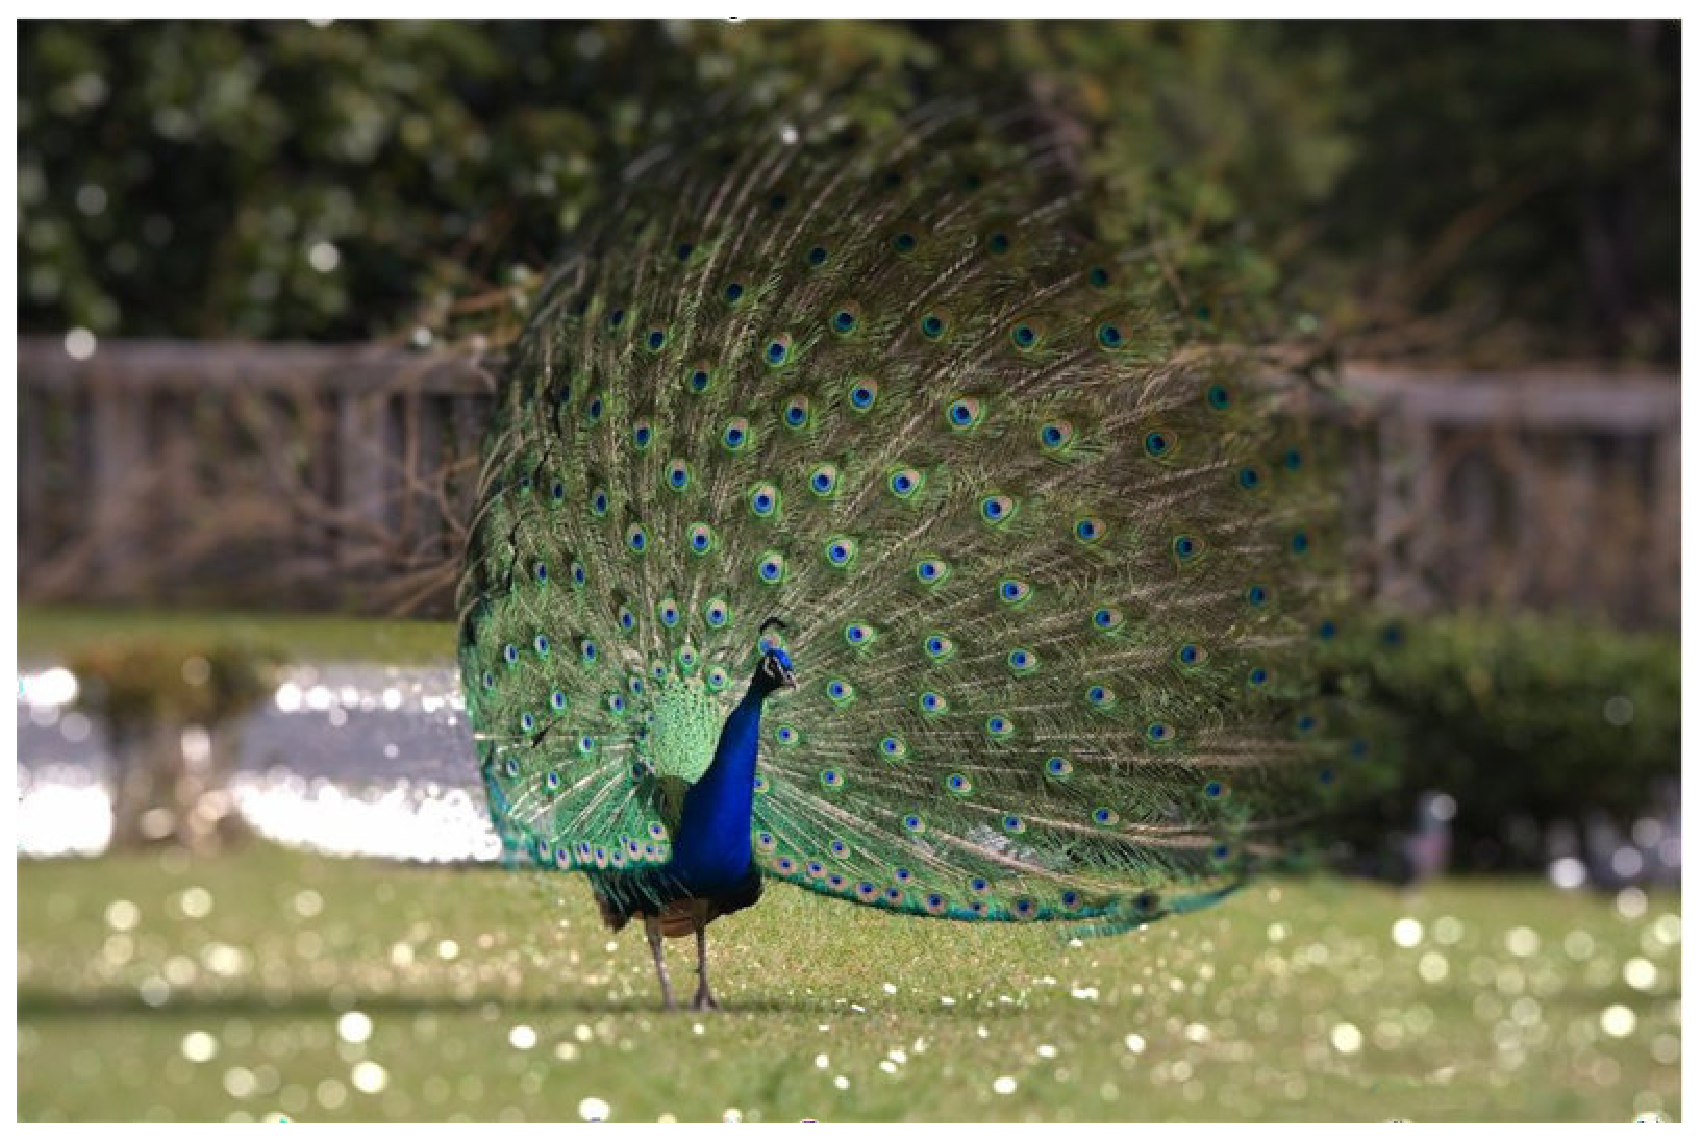
\includegraphics[width=0.45\columnwidth]{chapter-2/images/peacock}}\hfill{}

\caption{\label{fig:subfig-fauna}Fauna}

\end{figure}

\section{Tables}

The caption of tables must be placed before the table itself and not
after. As for figures, tables can have a short caption that is used
in the \textsf{List of Tables} section.

Academic publications, but also thesis, often use the so-called <<formal
table>>, an example of these particular style is showed in Table
\ref{tab:formal-table}

\begin{table}[h]
\centering{}\caption[Short caption of the table]{\label{tab:formal-table}Detailed caption of this beautiful table}
{\small{}}%
\begin{tabular}{ccccc}
\toprule 
 & \multicolumn{2}{c}{\textbf{Category}} &  & \tabularnewline
\cmidrule{2-3} 
 & \textbf{first} & \textbf{second} & \textbf{Number} & \textbf{Complexity}\tabularnewline
\midrule 
\textbf{Item A} & $\alpha$ & $\beta$ & $4$ & $\Omega\left(n\right)$\tabularnewline
\textbf{Item B} & $\gamma$ & $\delta$ & $2$ & $\Omega\left(n^{2}\right)$\tabularnewline
\bottomrule
\end{tabular}
\end{table}
To set this particular style, right click in a cell of the table then
\textsf{More} \textsf{\lyxarrow} \textsf{Settings} \textsf{\lyxarrow}
\textsf{Border}, here you can select the formal style.

\subsection{Wide tables}

Sometimes tables are too wide for the column's width of the page.
Rather than changing the table's content you can shrink it to fit
the available space. The font size will be smaller but this is, in
general, a good method to fix too wide tables such as Table \ref{tab:wide-table},
the result is showed in Table \ref{tab:wide-table-shrunk}.

\begin{table}[h]
\caption{\label{tab:wide-table}This table is very wide}

\centering{}%
\begin{tabular}{ccccc}
\toprule 
\textbf{Method} & \textbf{Parameter one} & \textbf{Parameter two} & \textbf{Parameter three} & \textbf{Parameter four}\tabularnewline
\midrule 
A & $1$ & $2$ & $3$ & $4$\tabularnewline
B & $5$ & $7$ & $9$ & $11$\tabularnewline
\bottomrule
\end{tabular}
\end{table}
\begin{table}[h]
\caption{\label{tab:wide-table-shrunk}This table is shrunk to fit the column's
width}

\centering{}\resizebox{\linewidth}{!}{%
\begin{tabular}{ccccc}
\toprule 
\textbf{Method} & \textbf{Parameter one} & \textbf{Parameter two} & \textbf{Parameter three} & \textbf{Parameter four}\tabularnewline
\midrule 
A & $1$ & $2$ & $3$ & $4$\tabularnewline
B & $5$ & $7$ & $9$ & $11$\tabularnewline
\bottomrule
\end{tabular}}
\end{table}
Another solution is to set the width of table's columns. To set it,
right click in a cell of the table then \textsf{More} \textsf{\lyxarrow}
\textsf{Settings} \textsf{\lyxarrow} \textsf{Table settings}, here
you can set the width.

\subsection{Space between rows}

Another common problem with tables is when rows of the table are too
close together, this problem is very frequent when rows contain mathematical
expressions such as Table \ref{tab:math-table}. With a simple command
it is possible to increase the space between rows as showed in Table
\ref{tab:math-table-big-rows}.

\begin{table}[h]
\caption{\label{tab:math-table}This table is a bit tight}

\centering{}%
\begin{tabular}{cc}
\toprule 
\textbf{Name} & \textbf{Formula}\tabularnewline
\midrule 
Gaussian integral & $\int_{0}^{+\infty}e^{-\frac{x^{2}}{2}}\text{dx}=\frac{1}{2}\sqrt{\frac{\pi}{2}}$\tabularnewline
Taylor series & $\sum_{n=0}^{\infty}\frac{f^{\left(n\right)}\left(a\right)}{n!}\left(x-a\right)^{n}$\tabularnewline
\bottomrule
\end{tabular}
\end{table}
\begin{table}[h]
\caption{\label{tab:math-table-big-rows}Math cheatsheet}

\centering{}\renewcommand*{\arraystretch}{1.5}%
\begin{tabular}{cc}
\toprule 
\textbf{Name} & \textbf{Formula}\tabularnewline
\midrule 
Gaussian integral & $ $$\int_{0}^{+\infty}e^{-\frac{x^{2}}{2}}\text{dx}=\frac{1}{2}\sqrt{\frac{\pi}{2}}$\tabularnewline
Taylor series & $\sum_{n=0}^{\infty}\frac{f^{\left(n\right)}\left(a\right)}{n!}\left(x-a\right)^{n}$\tabularnewline
\bottomrule
\end{tabular}
\end{table}

\section{Algorithms}

If you have to add some algorithms there is a dedicated \LyX{} environment.
As for tables, the caption of an algorithm must be placed before the
pseudo code of the algorithm, short captions can be used also for
algorithm. This placement of the caption may sound strange but is
justified by the fact that algorithms, but also tables, are read from
the top down, so the description must be placed before the content.
On the other side, figures are viewed like a painting, so the description
must be placed below the content.

\begin{algorithm}[h]
\begin{enumerate}
\item \caption[Short caption of the algorithm]{\label{alg:the-algorithm}Detailed caption of this complicated algorithm}
Wake up

\begin{enumerate}
\item drink a coffee
\item brush your teeth
\end{enumerate}
\item Go to work
\item Come back home
\item Go to sleep
\end{enumerate}
\end{algorithm}
Unfortunately \LyX{} does not support algorithm commands offered by
some \LaTeX{} packages (\texttt{\textbackslash If}, \texttt{\textbackslash While},
\ldots ) out of the box. It is possible to use custom modules to handle
those commands or use the 2.1 beta version that supports some of them
but, as for now, it is better to write directly \LaTeX{} code. This
template uses the \textsf{algorithmicx} package, refer to the manual
of that package (\url{http://www.ctan.org/pkg/algorithmicx}) for
the documentation of all the commands. Algorithm \ref{alg:best-algorithm-ever}
shows an example of the usage of some commands of the \textsf{algorithmicx}
package.

\begin{algorithm}[h]
\caption{\label{alg:best-algorithm-ever}Best algorithm ever}
\begin{algorithmic}[1]
	\State $s \gets \texttt{ALIVE}$ \Comment{Day of birth}
	\While{$ s \neq \texttt{EOL}$}
		\Repeat \Comment{Early morning, possibly}
			\State Try to wake up
		\Until{$s = \texttt{SLEEP}$}
		\State Drink a coffe \Comment{Even more than one}
		\State Brush your teeth
		\State Go to work \Comment{With a smile on your face}
		\State Come back home
		\State Go to sleep
	\EndWhile
\end{algorithmic}
\end{algorithm}

\section{Source code}

You may need to add some pieces of source code that you have written.
\LyX{} uses \textsf{listings} package to provide a customized environment
to insert source code (\textsf{Insert} \textsf{\lyxarrow{} Program
Listing}). Listings can have a caption, but \LyX{} does not add it
by default, if you want you can insert it (place the cursor inside
the listing environment, then \textsf{Insert \lyxarrow{} Caption}).

By default, the result that you get is pretty ugly as you can see
in the Listing \ref{lis:ugly-code}.

\begin{lstlisting}[caption={Program that computes your degree mark},label={lis:ugly-code}]
#include <stdlib.h>
#include <stdio.h>

/**
 * Main program
 */
int main(int argc, char *argv[])
{
	long double degree_mark = 0x42 * 042 * 0b00101010 * 0.001167;

	printf("Congratulations for your degree\n");
	printf("Your mark is %-3.0LfL\n", degree_mark);

	return EXIT_SUCCESS;
}
\end{lstlisting}

You need to set a couple of options (right click inside the source
code environment, then \textsf{Settings}) to get a good looking result.
The most important options are
\begin{description}
\item [{Font~style}] use a fixed-length font (\textsf{Font Family: Typewriter}),
it is useful to set a \textsf{Small} font size to compact large pieces
of source code. Breaking long lines is very important as well as hiding
nasty spaces (check \textsf{Break long lines} option, uncheck \textsf{Space
as symbol} and \textsf{Space in strings as symbol} options, set \textsf{Tabular
size} to $4$)
\item [{Line~numbering}] having the line numbering active is useful if
you have to refer to a particular statement when you are describing
you code
\item [{Language}] setting the proper language is important to have the
correct syntax highlighting
\end{description}
The Listing \ref{lis:beautiful-code} has the same code as the Listing
\ref{lis:ugly-code} but it has all the options mentioned before adjusted,
the result is way better that the other.

\begin{lstlisting}[caption={Program that computes your degree mark},label={lis:beautiful-code},basicstyle={\small\ttfamily},breaklines=true,commentstyle={\color{purple!60!black}},extendedchars=true,identifierstyle={\color{blue!50!black}},keywordstyle={\bfseries\color{green!50!black}},language=C,numbers=left,numberstyle={\footnotesize},showstringspaces=false,stringstyle={\color{orange!40!black}},tabsize=4,xleftmargin=2em]
#include <stdlib.h>
#include <stdio.h>

/**
 * Main program
 */
int main(int argc, char *argv[])
{
	long double degree_mark = 0x42 * 042 * 0b00101010 * 0.001167;

	printf("Congratulations for your degree\n");
	printf("Your mark is %-3.0LfL\n", degree_mark);

	return EXIT_SUCCESS;
}
\end{lstlisting}

If you have to insert more than one piece of code it can be useful
to copy the previously created environment and then modify it. This
saves you from setting the options every time you insert a new listing.

\section{URLs}

\LyX{} has a dedicated command to insert URLs (\textsf{Insert \lyxarrow{}
URL}) that must be used to insert each URL. The environment automatically
uses a typewrite font for the text, inserts a hyperlink to the URL
and, most importantly, breaks long URLs in multiple lines.

This is a URL added as simple text, http://this.is.not.the.correct.way.to.add.urls.in.lyx.documents.html.

This is a URL created with the \textsf{url} command, \url{http://this.is.the.correct.way.to.add.urls.in.lyx.documents.html}.

The \textsf{url} environment can be manually used, for example, in
the bibliography where URLs are not handled in a dedicated way. The
Listing \ref{lis:urls-bibliography} shows how to use the url command
in the bibliography.

\begin{lstlisting}[caption={How to insert URLs in the bibliography},label={lis:urls-bibliography},basicstyle={\small\ttfamily},breaklines=true,commentstyle={\color{purple!60!black}},extendedchars=true,identifierstyle={\color{blue!50!black}},keywordstyle={\bfseries\color{green!50!black}},language=TeX,numbers=left,numberstyle={\footnotesize},showstringspaces=false,stringstyle={\color{orange!40!black}},tabsize=4,xleftmargin=2em]
% this URL will not be broken into multiple lines and
% will NOT have a hyperlink
@article{
    ...
    howpublished = {http://google.com}
}

% this URL WILL be broken into multiple lines and
% WILL have a hyperlink
@article{
    ...
    howpublished = {\url{http://google.com}}
}
\end{lstlisting}


\section{\protect\LyX 's guides}

\LyX{} has a series of guides that describe all its features, if want
to exploit all the available functionalities you need to read them.
Those manuals are available directly in \LyX{} (for example, \textsf{Help}
\textsf{\lyxarrow{} Embedded Objects}).


\chapter{Third chapter\label{chap:third-chapter}}

These are very personal suggestions, no offense will be taken if you
completely ignore this chapter.

\section{Manage bibliography}

Manage a lot of bibliography resources by manually editing a \textsf{bibtex}
file is very annoying, it is better to use something that manages
for you all the references. Sadly, \LyX{} does not have an easy to
use system for doing that. However, there are other programs that
can be used to automagically organize dozens of papers.

There are two famous programs\textsf{, referencer} and \textsf{JabRef}
(\texttt{\url{https://launchpad.net/referencer},} \url{http://jabref.sourceforge.net/}),
both have a lot of useful features, the most notable are
\begin{itemize}
\item copy from clipboard of \textsf{bibtex} formatted references
\item organization of references with labels
\item possibility to associate a \textsf{pdf} to each reference
\item the \textsf{Cite in \LyX{} }button
\end{itemize}

\section{Reviews}

Your advisor will review what are you writing and he will, most likely,
add annotations on a \textsf{pdf}. However, correction contained inside
annotations are difficult to integrate, manly because you will spend
a lot of time in finding where to modify your document. \LyX{} supports
a very powerful method to review a document, just look the examples
below.

Where have you learned english stupid dumbass?

The derivative of $e^{x}$ is $e^{2x}$ .

After having considered all the other solutions we proved that this
is the most efficient way to determine the medium length of horse's
mane.

These result shows that the first method is way better than the second.
\\
The integration of these reviews is much easier than reviews inside
annotation of a \textsf{pdf}. Unfortunately you have to convince your
advisor to use this system, I think it is worth a try.

This feature is called \textsf{Change Tracking}, there is a dedicated
toolbar that you can show by activating the \textsf{Change Track}
option (\textsf{Document \lyxarrow{} Change Tracking \lyxarrow{} Track
Changes} or simply \textsf{CTRL + SHIFT + E}). This document has the
\textsf{Change Tracking} option already enabled.

\section{Final presentation}

Once you have written your thesis you will have to present it. Timing
is critical. You will have from $15$ to $20$ minutes to present
the work of months. A very useful tool that you may use during your
presentation is \texttt{pdfpc} (\url{http://davvil.github.io/pdfpc/}).
By using this program, on the screen of your laptop you will have
some additional information that are not showed on the external monitor.
These extra information are
\begin{description}
\item [{Time~left}] you can set the duration of the presentation and see
how many minutes and seconds you have left
\item [{Next~slide}] you will see both the current and the next slide
\item [{Annotations}] you can add some annotation to remember you some
key points that you may forget
\end{description}
This tool is very very useful, but do not forget that there is always
the demo effect. You MUST try it before even thinking to use for your
final presentation.

To install the program on a Linux system there should be a package
named \textsf{pdf-presenter-console}, for other OS on the websites
of the program there are the instruction how to install it.


\chapter{Fourth chapter\label{chap:fourth-chapter}}

These are style suggestions that you can use to personalize and beautify
your thesis.

\section{Font}

One important stylistic change that you can do is changing the font.
The default one is Computer Modern which is ok, but there are other
fonts that can be used. You can change the font in the properties
of the document (\textsf{Document} \textsf{\lyxarrow} \textsf{Settings}
\textsf{\lyxarrow} \textsf{Fonts}). Not all the fonts can be used
when compiling with \textsf{pdflatex}, with some fonts you need to
render the \textsf{pdf} with Xe\LaTeX{} or Lua\LaTeX . Figure \ref{fig:font-styles}
shows two different examples of fonts combination.

\begin{figure}[h]
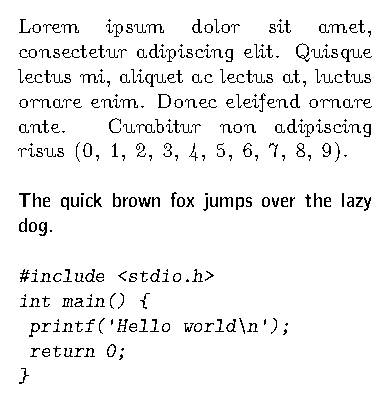
\includegraphics{chapter-4/images/latin-modern-font}\hfill{}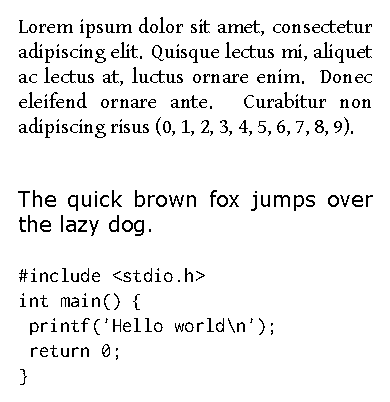
\includegraphics{chapter-4/images/funny-combination-font}

\caption{\label{fig:font-styles}Two different font styles}
\end{figure}
The fonts used in the example are summarized in the Table \ref{tab:font-names}.

\begin{center}
\begin{table}[h]
\centering{}\caption{\label{tab:font-names}Fonts used in the two examples showed before}
\begin{tabular}{lll}
\toprule 
\textbf{Serif} & Latin Modern Roman Unslanted & Gentium\tabularnewline
\textbf{Sans Serif} & Latin Modern Sans Demi Condensed & Verdana\tabularnewline
\textbf{Typewriter} & Latin Modern Mono Slanted & Inconsolata\tabularnewline
\bottomrule
\end{tabular}
\end{table}
\par\end{center}

If, by looking at the \textsf{pdf}, the letters look ugly check the
property of the \textsf{pdf}, in particular the type of fonts used
(how to find this information depends on the \textsf{pdf} viewer that
you are using, if you are using Linux use \textsf{pdffonts} command).
If your \textsf{pdf} has \textsf{Type 3} fonts that is the reason
why your \textsf{pd}f looks ugly. It is better to use \textsf{Type
1} fonts, if you are running \LyX{} on a Linux system by installing
\textsf{cm-super} package you can fix this problem.

\section{Fancy chapter header}

The header of each chapter can be personalized as you like, this requires
you to write a rather big amount of \LaTeX{} code to get a nice result.
However, there is package that provides a set of predefined styles,
\textsf{fncychap} (\url{http://www.ctan.org/pkg/fncychap}). Figure
\ref{fig:fancy-headers} shows just two of the styles offered by the
package.

\begin{center}
\begin{figure}[h]
\begin{centering}
\subfloat[Lenny style]{\centering{}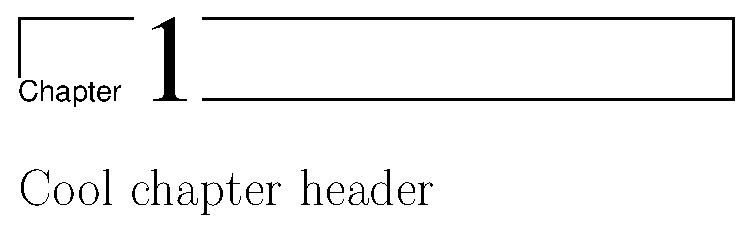
\includegraphics[width=0.6\columnwidth]{chapter-4/images/fancy-page-header-1}}
\par\end{centering}
\begin{centering}
\subfloat[Conny style]{\begin{centering}
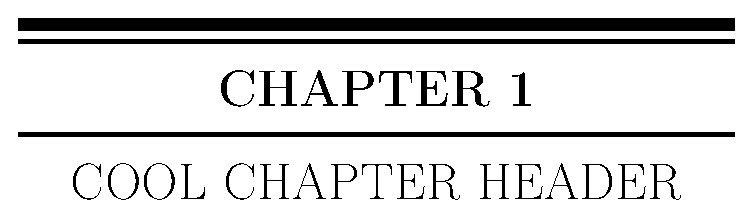
\includegraphics[width=0.6\columnwidth]{chapter-4/images/fancy-page-header-2}
\par\end{centering}
}
\par\end{centering}
\caption{\label{fig:fancy-headers}Two possible styles for headers of chapters}
\end{figure}
\par\end{center}

\section{Fancy initial letters}

Another thing that can be fancied are the initial letters. This is
a very simple modification that you can do to add a personal touch
to each chapter. There is a package that permits to customize, with
various options, initial letters called \textsf{lettrine} (\url{http://www.ctan.org/pkg/lettrine}).
There are a lot of options to create your personal style for each
initial, Figure \ref{fig:initial-letters} shows two possible styles
of initials.

\begin{center}
\begin{figure}[h]
\begin{centering}
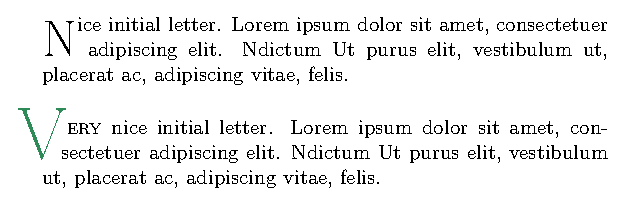
\includegraphics{chapter-4/images/lettrine}
\par\end{centering}
\caption{\label{fig:initial-letters}Two examples of initial letters}
\end{figure}
\par\end{center}

\section{Fancy headers}

Fancy headers are already used in this template, the package used
is \textsf{fancyhdr} (\textsf{\url{http://www.ctan.org/pkg/fancyhdr}}).
There are a lot of options, this template uses almost the standard
style for the header but you can change it. For example, you may move
the page numbering from the bottom header to the top header, or remove
the horizontal line in the header, or \ldots{} . In this template the
fancy header style is set in the \LaTeX{} preamble of the \textsf{thesis.lyx}
document (\textsf{Document} \textsf{\lyxarrow} \textsf{Settings}
\textsf{\lyxarrow} \textsf{\LaTeX{} Preamble}) and just before the
\textsf{Introduction} chapter.

\section{Other document classes}

This template uses the \textsf{book} class, there are some more advanced
classes that have a lot of cool features such as the one offered by
\textsf{koma-script} or \textsf{memoir} (\textsf{\url{http://www.ctan.org/pkg/koma-script}},
\textsf{\url{http://www.ctan.org/pkg/memoir}}).

\LyX{} supports a discrete number of those alternative classes, however
to fully exploit the additional functionalities offered by those classes
you have to write raw \LaTeX{} code. If you want to deeply customize
your thesis maybe it is better if you start considering to write it
directly in \LaTeX{} rather than using \LyX .


\chapter{Fifth chapter\label{chap:fifth-chapter}}

\input{chapter-5/chapter-5.tex}

\chapter{Sixth chapter\label{chap:sixth-chapter}}

\input{chapter-6/chapter-6.tex}

\chapter{Seventh chapter\label{chap:seventh-chapter}}

\input{chapter-7/chapter-7.tex}

\chapter{Eighth chapter\label{chap:eighth-chapter}}

\input{chapter-8/chapter-8.tex}

\chapter{Ninth chapter\label{chap:ninth-chapter}}

\input{chapter-9/chapter-9.tex}

\chapter*{Conclusions\label{chap:conclusion}}

\addcontentsline{toc}{chapter}{Conclusions}
\markboth{Conclusions}{Conclusions}\input{conclusions.tex}
\bibliographystyle{plain}
\bibliography{bibliography}
\addcontentsline{toc}{chapter}{Bibliography}

\appendix

\chapter{First appendix\label{app:first-appendix}}

\input{appendix-a/appendix-a.tex}

\chapter{Second appendix\label{app:second-appendix}}

\input{appendix-b/appendix-b.tex}

\chapter{Third appendix\label{app:third-appendix}}

\input{appendix-c/appendix-c.tex}\cleardoublepage
\end{document}
